\chapter{CYTO AI}
CYTO AI is the first fully web-based image labeling and classifying tool there is. Due to the web-based design no installation of databases or any configuration is needed to use all advantages of modern machine learning and convenient labeling. Further no data will be uploaded to any server, all data never leaves the browser which makes CYTO AI very performant and sets a high standard of privacy at the same time. The following sections shall explain how CYTO AI works and which techniques and architectures were used to build it.

\subsection{System overview}
First pictures need to be uploaded by clicking on the upload button, whole folders can be selected. Mind that also all images in subfolders will be uploaded. In order to categorize images, categories need to be created. That is possible by clicking on the plus icon in the categories list. After all necessary categories have been created images can be annotated. There are several was to annoate an image. It is possible to drag an image and drop it on the wished category. A different way is to click on one picture in order to select it an then use the keyboard to annotate the image. Following keys are supported:

\begin{itemize}
	\item \keystroke{ 1 } \keystroke{2} \keystroke{3} \keystroke{4} \keystroke{5} \keystroke{6} \keystroke{7}
	\keystroke{8} \keystroke{9} \keystroke{0} where \keystroke{1} is the first category in list.
	\item \keystroke{$\Leftarrow$} backslash to delete a given category
\end{itemize}

Further it is possible to navigate through all images with the arrow keys \keystroke{$\Uparrow$} to go up in row and 
 \keystroke{$\Downarrow$} to go down in row. Further \keystroke{$\Rightarrow$} to go right in column and \keystroke{$\Leftarrow$} to go left in column.


Also it is possible to blend out certain categories by clicking on the category, clicking another time will blend in the category. That gives the possibility to only show certain categories or to only show unlabeled images.
If all categories are blended out it is still possible to annotate using this category the new labeled image will stay visible.

If pictures were labeled it makes sense to sort them, this is possible by clicking the sort button. This improves the overview and makes reviewing labels easier. Uncategorized images will always appear at the top.

Another feature that improves the overview is the slider. The slider makes it possible to adjust the number of displayed images per row. 

If pictures have at least been labeled with two different categories it is possible to automatically categorize all unlabeled images by clicking the "fit" button. By that all unlabeled images will be given a category and a number will be shown under the image. This number is the probability an image belongs to the given category.

\begin{figure}[H]
	\centering
	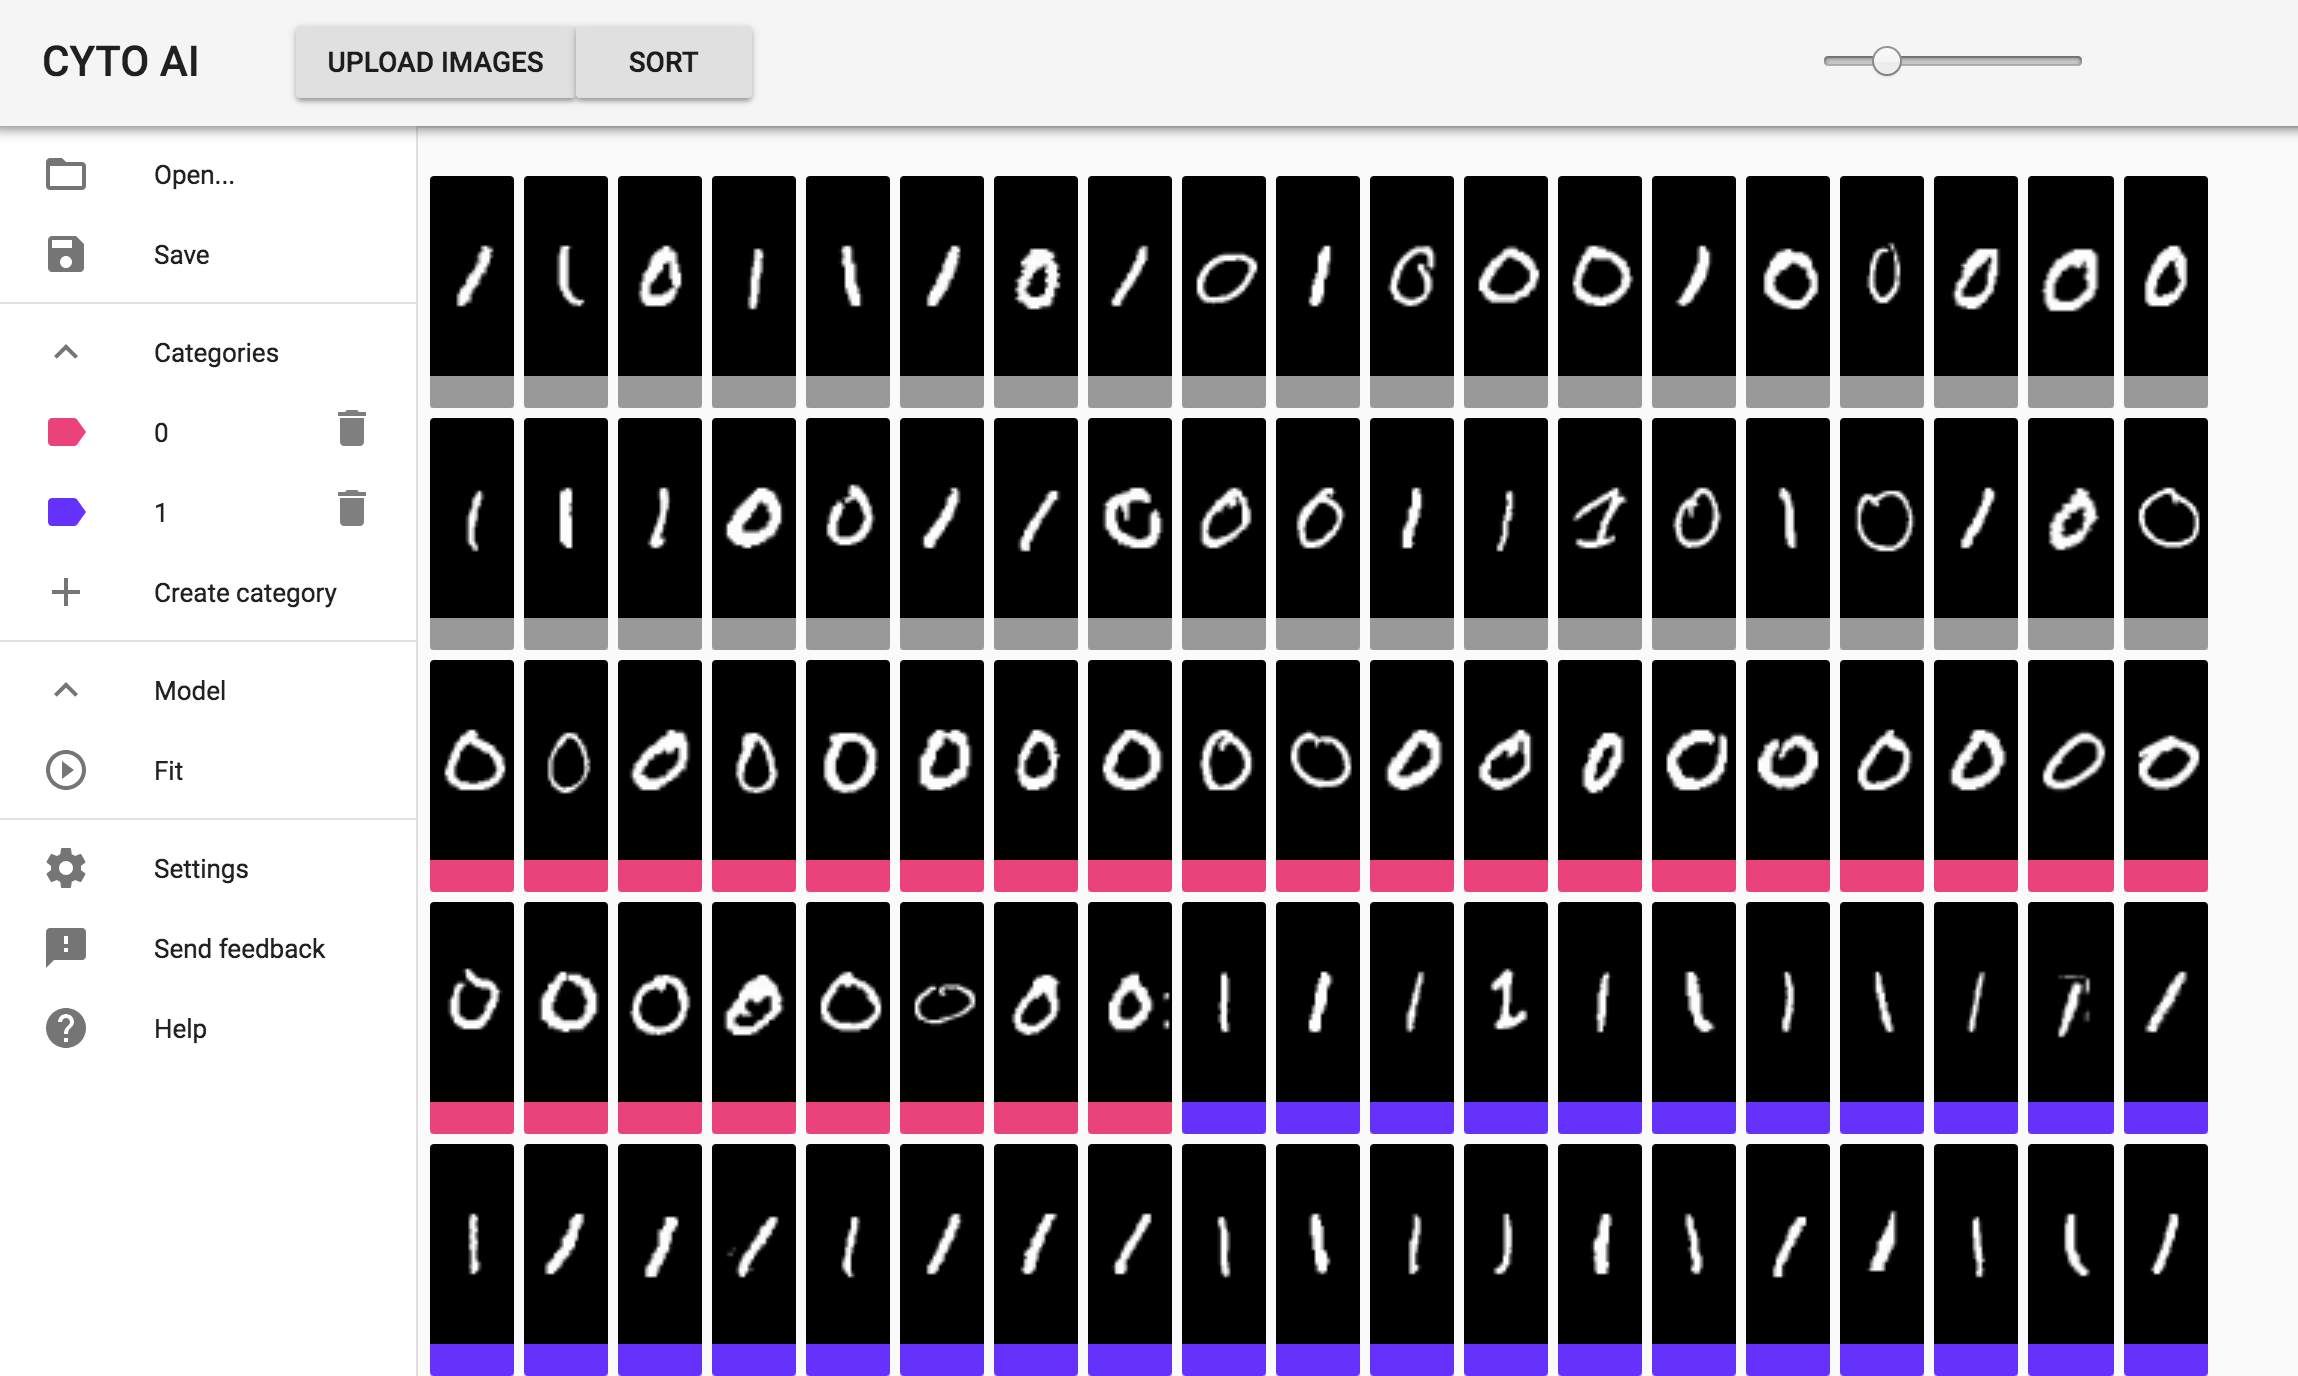
\includegraphics[width=0.8\linewidth]{bilder/cyto/cyto.png}
	\caption{CYOTO AI} source:\cite{Component}
	\label{fig:COMPONENT}
\end{figure}

To save all labels and categories and settings the button can be pressed. To import again the Open button can be used.


\subsection{System architecture}
CYTO AI is structured as tree of nested components. 

\begin{verbatim}
cyto
├── README.md
├── package-lock.json
├── package.json
├── src
│   ├── App.css
│   ├── App.js
│   ├── App.test.js
│   ├── actions
│   │   ├── categories.js
│   │   ├── categories.test.js
│   │   ├── classifier.js
│   │   ├── classifier.test.js
│   │   ├── images.js
│   │   ├── images.test.js
│   │   ├── settings.js
│   │   └── settings.test.js
│   ├── classifier.js
│   ├── components
│   │   ├── Categories.css.js
│   │   ├── Categories.js
│   │   ├── Categories.test.js
│   │   ├── Category.css.js
│   │   ├── Category.js
│   │   ├── Category.test.js
│   │   ├── Classifier.css.js
│   │   ├── Classifier.js
│   │   ├── Classifier.test.js
│   │   ├── CreateCategoryDialog.css.js
│   │   ├── CreateCategoryDialog.js
│   │   ├── CreateCategoryDialog.test.js
│   │   ├── Gallery.css.js
│   │   ├── Gallery.js
│   │   ├── Gallery.test.js
│   │   ├── HelpDialog.css.js
│   │   ├── HelpDialog.js
│   │   ├── HelpDialog.test.js
│   │   ├── Image.css.js
│   │   ├── Image.js
│   │   ├── Image.test.js
│   │   ├── Images.css
│   │   ├── Images.js
│   │   ├── Images.test.js
│   │   ├── Primary.css.js
│   │   ├── Primary.js
│   │   ├── Primary.test.js
│   │   ├── Settings.css.js
│   │   ├── Settings.js
│   │   ├── Settings.test.js
│   │   ├── Sidebar.css.js
│   │   ├── Sidebar.js
│   │   ├── Sidebar.test.js
│   │   ├── UploadButton.js
│   │   └── dnd-global-context.js
│   ├── constants.js
│   ├── containers
│   │   ├── ConnectedCategories.js
│   │   ├── ConnectedCategory.js
│   │   ├── ConnectedClassifier.js
│   │   ├── ConnectedCreateCategoryDialog.js
│   │   ├── ConnectedGallery.js
│   │   ├── ConnectedImage.js
│   │   ├── ConnectedImages.js
│   │   ├── ConnectedPrimary.js
│   │   ├── ConnectedSidebar.js
│   │   └── ConnectedUploadButton.js
│   ├── images
│   │   ├── mnist.json
│   │   └── stock.json
│   ├── index.css
│   ├── index.js
│   ├── reducers
│   │   ├── categories.js
│   │   ├── categories.test.js
│   │   ├── classifier.js
│   │   ├── classifier.test.js
│   │   ├── images.js
│   │   ├── images.test.js
│   │   ├── index.js
│   │   ├── settings.js
│   │   └── settings.test.js
│   ├── registerServiceWorker.js
│   ├── selectors
│   │   ├── images.js
│   │   ├── images.test.js
│   │   └── index.js
│   └── stories
│       └── index.js
└── yarn.lock

8 directories, 80 files

\end{verbatim}




\subsubsection{Component structure}

\subsubsection{Machine Learning API}

\subsection{Performance}

\subsection{Future perspective}




